\documentclass[tikz,border=10pt]{standalone}
\usepackage{tikz}
%setup Tikz to draw the graphs
%load options
\usetikzlibrary{positioning, calc, shapes.geometric, shapes.multipart,
        shapes, arrows.meta, arrows, decorations.markings, external, trees}

%Create custom arrow style:
\tikzstyle{Arrow} = [
thick,
decoration={
markings,
mark=at position 0.9999 with {
\arrow[thick]{latex}}},
shorten >= 3pt, preaction = {decorate}]

\begin{document}
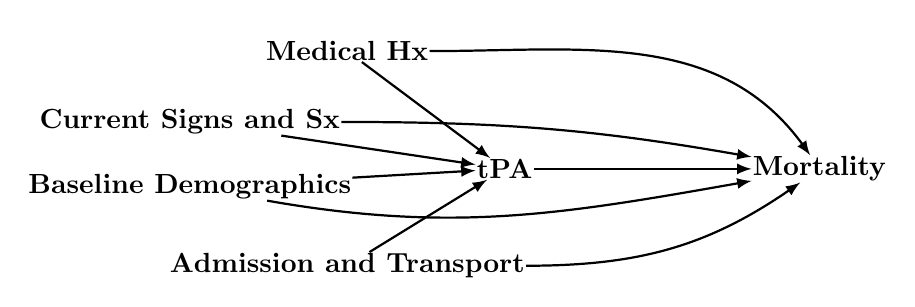
\begin{tikzpicture}
    \node [inner sep=0.1mm](1) at (1,-0.083){\textbf{Mortality}};
    \node [inner sep=0.1mm](2) at (-3,-0.083){\textbf{tPA}};
    \node [inner sep=0.1mm](3) at (-5,-1.313){\textbf{Admission and Transport}};
    \node [inner sep=0.1mm](4) at (-7,-0.313){\textbf{Baseline Demographics}};
    \node [inner sep=0.1mm](5) at (-7,0.513){\textbf{Current Signs and Sx}};
    \node [inner sep=0.1mm](6) at (-5,1.413){\textbf{Medical Hx}};
    
    \draw [Arrow] (2) to (1);
    \draw [Arrow] (3) to (2);
    \draw [Arrow] (4) to (2);
    \draw [Arrow] (5) to (2);
    \draw [Arrow] (6) to (2);

    \draw [Arrow] (6) to [out=0, in =125] (1);
    \draw [Arrow] (5) to [out=0, in =170] (1);
    \draw [Arrow] (4) to [out=-10, in=-170] (1);
    \draw [Arrow] (3) to [out=0, in=-145] (1);
\end{tikzpicture}
\end{document}

%command to convert graph to image
%magick -density 600 dag.pdf dag.png

% dag {
% "Admission and Transport" [pos="-0.879,0.110"]
% "Baseline Demographics" [pos="-1.163,0.016"]
% "Current Signs/Sx" [pos="-0.892,-0.148"]
% "Medical Hx" [pos="-1.145,-0.416"]
% "in hospital all cause mortality" [outcome,pos="-0.209,-0.083"]
% tPA [exposure,pos="-0.623,-0.085"]
% "Admission and Transport" -> "in hospital all cause mortality"
% "Admission and Transport" -> tPA
% "Baseline Demographics" -> "in hospital all cause mortality"
% "Baseline Demographics" -> tPA
% "Current Signs/Sx" -> "in hospital all cause mortality"
% "Current Signs/Sx" -> tPA
% "Medical Hx" -> "in hospital all cause mortality"
% "Medical Hx" -> tPA
% tPA -> "in hospital all cause mortality"
% }




% Daggity code:
% dag {
% "Rankin scale" [pos="-0.893,-0.148"]
% "admit type" [pos="-0.809,-0.492"]
% "cardiac illness hx" [pos="-1.318,-0.540"]
% "in hospital all cause mortality" [outcome,pos="0.000,-0.067"]
% "previous stroke" [pos="-1.501,0.569"]
% "time to admit" [pos="-0.659,-0.679"]
% "transport type" [pos="-0.957,0.512"]
% HTN [pos="-0.890,0.042"]
% afib [pos="-0.854,0.223"]
% age [pos="-1.053,-0.715"]
% aphasia [pos="-0.734,0.295"]
% consciousness [pos="-1.158,0.009"]
% diabetes [pos="-0.562,0.337"]
% gender [pos="-0.889,-0.323"]
% paresis [pos="-0.779,-0.932"]
% tPA [exposure,pos="-0.623,-0.085"]
% "Rankin scale" -> "in hospital all cause mortality"
% "Rankin scale" -> tPA
% "admit type" -> "in hospital all cause mortality"
% "admit type" -> tPA
% "cardiac illness hx" -> "in hospital all cause mortality"
% "cardiac illness hx" -> tPA
% "previous stroke" -> "in hospital all cause mortality"
% "previous stroke" -> tPA
% "time to admit" -> "in hospital all cause mortality"
% "time to admit" -> tPA
% "transport type" -> "in hospital all cause mortality"
% "transport type" -> tPA
% HTN -> "in hospital all cause mortality"
% HTN -> tPA
% afib -> "in hospital all cause mortality"
% afib -> tPA
% age -> "in hospital all cause mortality"
% age -> tPA
% aphasia -> "in hospital all cause mortality"
% aphasia -> tPA
% consciousness -> "in hospital all cause mortality"
% consciousness -> tPA
% diabetes -> "in hospital all cause mortality"
% diabetes -> tPA
% gender -> "in hospital all cause mortality"
% gender -> tPA
% paresis -> "in hospital all cause mortality"
% paresis -> tPA
% tPA -> "in hospital all cause mortality"
% }
